\documentclass[10pt]{article}
\usepackage[T1]{fontenc}

% Document Details
\newcommand{\CLASS}{AMATH 586}
\newcommand{\assigmentnum}{Assignment 1}

\usepackage[margin = 1.15in, top = 1.25in, bottom = 1.in]{geometry}

\usepackage{titling}
\setlength{\droptitle}{-6em}   % This is your set screw
\date{}
\renewcommand{\maketitle}{
	\clearpage
	\begingroup  
	\centering
	\LARGE \sffamily\textbf{\CLASS} \Large \assigmentnum\\[.8em]
	\large Tyler Chen\\[1em]
	\endgroup
	\thispagestyle{empty}
}
 % Title Styling
\usepackage{tocloft}
\renewcommand{\cfttoctitlefont}{\Large\sffamily\bfseries}
\renewcommand{\cftsecfont}{\normalfont\sffamily\bfseries}
\renewcommand{\cftsubsecfont}{\normalfont\sffamily}
\renewcommand{\cftsubsubsecfont}{\normalfont\sffamily}

\makeatletter
\let\oldl@section\l@section
\def\l@section#1#2{\oldl@section{#1}{\sffamily\bfseries#2}}

\let\oldl@subsection\l@subsection
\def\l@subsection#1#2{\oldl@subsection{#1}{\sffamily#2}}

\let\oldl@subsubsection\l@subsubsection
\def\l@subsubsection#1#2{\oldl@subsubsection{#1}{\sffamily#2}}
 % General Styling


\usepackage{enumitem}

% Figures
\usepackage{subcaption}

% TikZ and Graphics
\usepackage{tikz, pgfplots}
\pgfplotsset{compat=1.12}
\usetikzlibrary{patterns,arrows}
\usepgfplotslibrary{fillbetween}

\usepackage{pdfpages}
\usepackage{adjustbox}

\usepackage{lscape}
\usepackage{titling}
\usepackage[]{hyperref}


% Header Styling
\usepackage{fancyhdr}
\pagestyle{fancy}
\lhead{\sffamily \CLASS}
\rhead{\sffamily Chen \textbf{\thepage}}
\cfoot{}

% Paragraph Styling
\setlength{\columnsep}{1cm}
\setlength{\parindent}{0pt}
\setlength{\parskip}{5pt}
\renewcommand{\baselinestretch}{1}

% TOC Styling
\usepackage{tocloft}
\iffalse
\renewcommand{\cftsecleader}{\cftdotfill{\cftdotsep}}

\renewcommand\cftchapafterpnum{\vskip6pt}
\renewcommand\cftsecafterpnum{\vskip10pt}
\renewcommand\cftsubsecafterpnum{\vskip6pt}

% Adjust sectional unit title fonts in ToC
\renewcommand{\cftchapfont}{\sffamily}
\renewcommand{\cftsecfont}{\bfseries\sffamily}
\renewcommand{\cftsecnumwidth}{2em}
\renewcommand{\cftsubsecfont}{\sffamily}
\renewcommand{\cfttoctitlefont}{\hfill\bfseries\sffamily\MakeUppercase}
\renewcommand{\cftaftertoctitle}{\hfill}

\renewcommand{\cftchappagefont}{\sffamily}
\renewcommand{\cftsecpagefont}{\bfseries\sffamily}
\renewcommand{\cftsubsecpagefont}{\sffamily}
\fi
 % General Styling
% Code Display Setup
\usepackage{listings,lstautogobble}
\usepackage{lipsum}
\usepackage{courier}
\usepackage{catchfilebetweentags}

\lstset{
	basicstyle=\small\ttfamily,
	breaklines=true, 
	frame = single,
	rangeprefix=,
	rangesuffix=,
	includerangemarker=false,
	autogobble = true
}


\usepackage{algorithmicx}
\usepackage{algpseudocode}

\newcommand{\To}{\textbf{to}~}
\newcommand{\DownTo}{\textbf{downto}~}
\renewcommand{\algorithmicdo}{\hspace{-.2em}\textbf{:}}
 % Code Display Setup
% AMS MATH Styling
\usepackage{amsmath, amssymb}
\newcommand{\qed}{\hfill\(\square\)}

%\newtheorem*{lemma}{Lemma} 
%\newtheorem*{theorem}{Theorem}
%\newtheorem*{definition}{Definition}
%\newtheorem*{prop}{Proposition}
%\renewenvironment{proof}{{\bfseries Proof.}}{}


% mathcal
\newcommand{\cA}{\ensuremath{\mathcal{A}}}
\newcommand{\cB}{\ensuremath{\mathcal{B}}}
\newcommand{\cC}{\ensuremath{\mathcal{C}}}
\newcommand{\cD}{\ensuremath{\mathcal{D}}}
\newcommand{\cE}{\ensuremath{\mathcal{E}}}
\newcommand{\cF}{\ensuremath{\mathcal{F}}}
\newcommand{\cG}{\ensuremath{\mathcal{G}}}
\newcommand{\cH}{\ensuremath{\mathcal{H}}}
\newcommand{\cI}{\ensuremath{\mathcal{I}}}
\newcommand{\cJ}{\ensuremath{\mathcal{J}}}
\newcommand{\cK}{\ensuremath{\mathcal{K}}}
\newcommand{\cL}{\ensuremath{\mathcal{L}}}
\newcommand{\cM}{\ensuremath{\mathcal{M}}}
\newcommand{\cN}{\ensuremath{\mathcal{N}}}
\newcommand{\cO}{\ensuremath{\mathcal{O}}}
\newcommand{\cP}{\ensuremath{\mathcal{P}}}
\newcommand{\cQ}{\ensuremath{\mathcal{Q}}}
\newcommand{\cR}{\ensuremath{\mathcal{R}}}
\newcommand{\cS}{\ensuremath{\mathcal{S}}}
\newcommand{\cT}{\ensuremath{\mathcal{T}}}
\newcommand{\cU}{\ensuremath{\mathcal{U}}}
\newcommand{\cV}{\ensuremath{\mathcal{V}}}
\newcommand{\cW}{\ensuremath{\mathcal{W}}}
\newcommand{\cX}{\ensuremath{\mathcal{X}}}
\newcommand{\cY}{\ensuremath{\mathcal{Y}}}
\newcommand{\cZ}{\ensuremath{\mathcal{Z}}}

% mathbb
\usepackage{bbm}
\newcommand{\bOne}{\ensuremath{\mathbbm{1}}}

\newcommand{\bA}{\ensuremath{\mathbb{A}}}
\newcommand{\bB}{\ensuremath{\mathbb{B}}}
\newcommand{\bC}{\ensuremath{\mathbb{C}}}
\newcommand{\bD}{\ensuremath{\mathbb{D}}}
\newcommand{\bE}{\ensuremath{\mathbb{E}}}
\newcommand{\bF}{\ensuremath{\mathbb{F}}}
\newcommand{\bG}{\ensuremath{\mathbb{G}}}
\newcommand{\bH}{\ensuremath{\mathbb{H}}}
\newcommand{\bI}{\ensuremath{\mathbb{I}}}
\newcommand{\bJ}{\ensuremath{\mathbb{J}}}
\newcommand{\bK}{\ensuremath{\mathbb{K}}}
\newcommand{\bL}{\ensuremath{\mathbb{L}}}
\newcommand{\bM}{\ensuremath{\mathbb{M}}}
\newcommand{\bN}{\ensuremath{\mathbb{N}}}
\newcommand{\bO}{\ensuremath{\mathbb{O}}}
\newcommand{\bP}{\ensuremath{\mathbb{P}}}
\newcommand{\bQ}{\ensuremath{\mathbb{Q}}}
\newcommand{\bR}{\ensuremath{\mathbb{R}}}
\newcommand{\bS}{\ensuremath{\mathbb{S}}}
\newcommand{\bT}{\ensuremath{\mathbb{T}}}
\newcommand{\bU}{\ensuremath{\mathbb{U}}}
\newcommand{\bV}{\ensuremath{\mathbb{V}}}
\newcommand{\bW}{\ensuremath{\mathbb{W}}}
\newcommand{\bX}{\ensuremath{\mathbb{X}}}
\newcommand{\bY}{\ensuremath{\mathbb{Y}}}
\newcommand{\bZ}{\ensuremath{\mathbb{Z}}}

% alternative mathbb
\newcommand{\NN}{\ensuremath{\mathbb{N}}}
\newcommand{\RR}{\ensuremath{\mathbb{R}}}
\newcommand{\CC}{\ensuremath{\mathbb{C}}}
\newcommand{\ZZ}{\ensuremath{\mathbb{Z}}}
\newcommand{\EE}{\ensuremath{\mathbb{E}}}
\newcommand{\PP}{\ensuremath{\mathbb{P}}}
\newcommand{\VV}{\ensuremath{\mathbb{V}}}
\newcommand{\cov}{\ensuremath{\text{Co}\VV}}
% Math Commands

\newcommand{\st}{~\big|~}
\newcommand{\stt}{\text{ st. }}
\newcommand{\ift}{\text{ if }}
\newcommand{\thent}{\text{ then }}
\newcommand{\owt}{\text{ otherwise }}

\newcommand{\norm}[1]{\left\lVert#1\right\rVert}
\newcommand{\snorm}[1]{\lVert#1\rVert}
\newcommand{\ip}[1]{\ensuremath{\left\langle #1 \right\rangle}}
\newcommand{\pp}[3][]{\frac{\partial^{#1}#2}{\partial #3^{#1}}}
\newcommand{\dd}[3][]{\frac{\d^{#1}#2}{\d #3^{#1}}}
\renewcommand{\d}{\ensuremath{\mathrm{d}}}

\newcommand{\indep}{\rotatebox[origin=c]{90}{$\models$}}




 % Math shortcuts
% Problem
\usepackage{floatrow}

\newenvironment{problem}[1][]
{\pagebreak
\noindent\rule{\textwidth}{1pt}\vspace{0.25em}
{\sffamily \textbf{#1}}
\par
}
{\par\vspace{-0.5em}\noindent\rule{\textwidth}{1pt}}

\newenvironment{solution}[1][]
{{\sffamily \textbf{#1}}
\par
}
{}

 % Problem Environment

\newcommand{\note}[1]{\textcolor{red}{\textbf{Note:} #1}}

\hypersetup{
   colorlinks=true,       % false: boxed links; true: colored links
   linkcolor=violet,          % color of internal links (change box color with linkbordercolor)
   citecolor=green,        % color of links to bibliography
   filecolor=magenta,      % color of file links
   urlcolor=cyan           % color of external links
}


\begin{document}
\maketitle



\begin{problem}[Problem 1]
Prove that the ODE IVP
\[
u' (t) = \frac{1}{t^2 + 2 u(t )^2} ,~~~ t \geq 1 ,
\]
\[
u(1) = \eta ,
\]
has a unique solution for all \( t \geq 1 \).  Find an optimal or near optimal Lipschitz constant
for this problem.
\end{problem}

\begin{solution}[Solution]
Write \( f(u,t) = 1/(t^2+2u^2) \). Then,
\begin{align*}
    \pp{f}{u} = -\dfrac{4 u}{(t^2+2u^2)^2}
\end{align*}

We now maximize \( |f_u(u,t)| \) with respect to \( u \).
We have,
\begin{align*}
    \pp[2]{f}{u} = \frac{32 u^2}{\left(t^2+2 u^2\right)^3}-\frac{4}{\left(t^2+2 u^2\right)^2}
\end{align*}

Clearly \( f_{uu} = 0 \) at \( u = \pm t / \sqrt{6} \). We can easily check that both these points maximize \( |f_u(u,t)| \). Therefore, since \( f_u \) is a decreasing function of \( t \) , for any domain,
\begin{align*}
    \cD = \{(u,t) : |u-\eta| \leq a, t_0 \leq t \leq t_1 \}
\end{align*}
we have Lipschitz constant,
\begin{align*}
    L = \dfrac{\sqrt{3^3/2^5}}{t_0^3}
\end{align*}

Therefore, by a theorem from the book, the ODE IVP has a unique solution at least up to time,
\begin{align*}
    T^* = \min\{ t_1,t_0 + a/S \}, && S = \max_{(u,t)\in \cD} |f(u,t)|
\end{align*}

Observe that,
\begin{align*}
    S = \max_{t\geq 1} |f(u,t)|
    \leq \max_{t\geq 1} \left|\dfrac{1}{t^2}\right|
    = 1
\end{align*}
and that if \( u = 0 \) this inequality is tight.

Therefore, for any domain \( \cD \) of the form above, \( t_0 + a/S \geq t_0 + a \).

Let \( t\geq 1 \). Pick \( t_0 = 1 \), \( t_1 > t \), and \( a > t-1 \) so that,
\begin{align*}
    \min\{t_1, t_0 + a/S\} > t
\end{align*}
Then there is a unique solution to the ODE IVP up to time \( T^* > t \). This proves that the ODE IVP has a unique solution for all time \( t\geq 1 \).
For domains of this form we have Lipschitz constant,
\begin{align*}
    L = \sqrt{\dfrac{3^3}{2^5}}
\end{align*}

This constant is optimal since the derivative is continuous. To see this consider the expansion of \( f_u(t_0/\sqrt{6}+h,t_0) \) about \( (t_0/\sqrt{0},t_0) \). Clearly this can be made arbitrarily close to \( L \) by picking \( h \) sufficiently small. This means that for any \( l < L \), there is some interval for which \( |f_u(t_0/\sqrt{6}, t_0) - f_u(t_0/\sqrt{6}+h,t_0)| > l |u_0+h-u_0| \). That is, \( l \) is not a Lipschitz constnat for \( f \) with respect to \( u \).
 \qed

\end{solution}

\begin{problem}[Problem 2]
Consider the equation of harmonic motion:
\[
u'' = - k u ,~~~u( t_0 ) = u_0 ,~~~u' ( t_0 ) = v_0 .
\]
Here \( u(t) \) represents the distance from equilibrium and \( k > 0 \) is a spring constant.
Write this as a system of two first-order differential equations, and show that the
right-hand side of your system satisfies a Lipschitz condition on \( {\bf R}^2 \).  Determine
the (smallest possible) Lipschitz constant for the 1-norm, the 2-norm, and the \( \infty \)-norm.
(See Appendix A.3.)
\end{problem}

\begin{solution}[Solution]

Define \( v = u' \). Then \( v' = u'' \) so the original equation can be written as,
\begin{align*}
    \begin{cases}
        v' = - k u \\
        u' = v,
    \end{cases}
    &&
    \begin{cases}
        u(t_0) = u_0 \\
        v(t_0) = v_0
    \end{cases}
\end{align*}

We now show that the right hand side is uniformly Lipschitz by finding Lipschitz constants for the 1-norm, 2-norm, and the \( \infty \)-norm.
Write,
\begin{align*}
    x = \left[\begin{array}{c} v \\ u\end{array}\right], && f(x) = \left[\begin{array}{c}-ku \\ v\end{array}\right]
\end{align*}

Define the indicator function \( \mathbbm{1}:\{\verb|true|,\verb|false|\}\to\{0,1\} \) by \( \mathbbm{1}[\varphi] = \{ 1 : \varphi = \verb|true|,~ 0: \varphi = \verb|false| \} \). Observe that,
\begin{align*}
    \left[\begin{array}{c}-ku \\ v\end{array}\right] = \max\{k,1\}\left[\begin{array}{c}-u \\ v\end{array}\right] + \left[\begin{array}{c} (1-k)\mathbbm{1}[k\leq1] u \\ (1-k)\mathbbm{1}[k>1]v \end{array}\right]
\end{align*}

Let \( \tilde{x} = x - x^* \).
Note that \( k \) is linear so that for any \( x,x^* \), \( f(x) - f(x^*) = f(x-x^*) = f(\tilde{x}) \).
Therefore, for any norm \( \norm{\cdot} \), by the triangle inequality,
\begin{align*}
    \norm{f(\tilde{x})} \leq \max\{k,1\}\norm{\tilde{x}}
\end{align*}

Note that \( \tilde{x} = [\mathbbm{1}[k\geq 1], \mathbbm{1}[k < 1]] \) attains the bound above.
This proves that \( \max\{k,1\} \) is the optimal Lipschitz constant for any norm. \qed

\end{solution}

\begin{problem}[Problem 3]
Consider the one-step method
\[
U^{n+1} = U^n + k [ \theta f( U^n , t_n ) + (1 - \theta ) f ( U^{n+1} , t_{n+1} ) ] ,
\]
where \( \theta \in [0,1] \) is given.  Note that this method is {\em explicit} if \( \theta = 1 \)
and otherwise it is implicit.  Show that the local truncation error is \( O( k^2 ) \) if \( \theta = 1/2 \)
and otherwise it is \( O(k) \).
\end{problem}

\begin{solution}[Solution]

Note,
\begin{align*}
    f(u(t_n),t_n) = u'(t_n), && f(u(t_{n+1}),t_{n+1}) = u'(t_{n+1})
\end{align*}


We expand,
\begin{align*}
    u(t_{n+1}) &= u(t_n) + u'(t_n)k + \dfrac{1}{2!}u''(t_n)k^2 + \dfrac{1}{3!}u'''(t_n)k^3 + \cO(k^4) \\
    u'(t_{n+1}) &= u'(t_n) + u''(t_n)k + \dfrac{1}{2!}u'''(t_n)k^2 + \dfrac{1}{3!}u''''(t_n)k^3 + \cO(k^4) \\
\end{align*}

Therefore,
\begin{align*}
    \dfrac{1}{k} \left( u(t_{n+1}) - u(t_n) \right) &= u'(t_n) + \dfrac{1}{2!}u''(t_n)k + \dfrac{1}{3!} u'''(t_n)k^2 + \cO(k^3) \\
    \theta u'(t_n) + (1-\theta) u'(t_{n+1}) &= u'(t_n) + (1-\theta)\left( u''(t_n)k + \dfrac{1}{2!}u'''(t_n)k^2 + \cO(k^3) \right)
\end{align*}

We have local truncation error,
\begin{align*}
    \tau^n &= \dfrac{1}{k} \left( u(t_{n+1})-u(t_n) \right) - \theta f(u(t_n),t_n) - (1-\theta) f(u(t_{n+1}),t_{n+1})
    \\&= \left( \dfrac{1}{2!}u''(t_n)k + \dfrac{1}{3!}u'''(t_n)k^2 + \cO(k^3) \right) - (1-\theta) \left( u''(t_n)k + \dfrac{1}{2!}u'''(t_n)k^2 + \cO(k^3) \right)
\end{align*}

Clearly the \( \cO(k) \) terms cancel if and only if \( \theta = 1/2 \), in which case the leading order terms are \( \cO(k^2) \). Otherwise the leading order terms are \( \cO(k) \). \qed

\end{solution}

\begin{problem}[Problem 4]
Compute the leading term in the local truncation error of the following methods:
\begin{enumerate}[label=(\alph*)]
\item
Heun's method:
\begin{eqnarray*}
\tilde{U}^{n+1} & = & U^n + k f( U^n , t_n ) , \\
U^{n+1} & = & U^n + \frac{k}{2} \left[ f( \tilde{U}^{n+1}, t_{n+1} ) + f( U^n , t_n ) \right] .
\end{eqnarray*}
\item
The Runge-Kutta method (5.32).
\begin{eqnarray*}
    \tilde{U}^{n+1} & = & U^n + \frac{1}{2}k f( U^n , t_n ) , \\
U^{n+1} & = & U^n + k f\left( \tilde{U}^{n+1}, t_{n} + \dfrac{k}{2} \right)
\end{eqnarray*}
\end{enumerate}
\end{problem}

\begin{solution}[Solution]

\begin{enumerate}[label=(\alph*)]
    \item
        We expand,
        \begin{align*}
            u(t + k) &= u(t) + u'(t)k + \dfrac{1}{2!}u''(t)k^2 + \dfrac{1}{3!}u'''(t)k^3 + \cO(k^4)
        \end{align*}

        Similarly, in two dimensions,
        \begin{align*}
            f(u + k u', t+k)
            &= f(u,t) + f_u(u,t)u' k + f_t(u,t)k
            \\& \hspace{2em}+ \dfrac{1}{2!} \Big( f_{uu}(u,t)u'^2k^2 + 2f_{ut}(u,t)u'k^2 + f_{tt}(u,t)k^2 \Big) + \cO(k^3)
        \end{align*}

        Now observe that by the limit definition of the derivative,
        \begin{align*}
            u'' = \pp{}{t} u' = \pp{}{t} f(u,t) = f_u(u,t)u' + f_t(u,t)
        \end{align*}

        We can therefore write,
        \begin{align*}
            f(u + k u',t+k)
            &= u' + u'' k + \dfrac{1}{2!} \left( f_{uu}(u,t)u'^2k^2 + 2f_{ut}(u,t)u'k^2 + f_{tt}(u,t)k^2 \right) + \cO(k^3)
            \end{align*}

        Using the fact that \( f(u(t_n)) = u'(t_n)  \),
        \begin{align*}
            \dfrac{1}{k} \left( u(t_{n+1}) - u(t_n) \right) &= u'(t_n) + \dfrac{1}{2}u''(t_n)k + \dfrac{1}{3!}u'''(t_n)k^2 + \cO(k^3) \\
            f(u(t_n) + kf(u(t_n))) + f(u(t_n)) &=
            2u'(t_n) + u''(t_n) k
            + \dfrac{1}{2!} \big( f_{uu}(u(t_n),t_n)u'(t_n)^2
            \\&\hspace{2em} + 2f_{ut}(u(t_n),t_n)u'(t_n)
            + f_{tt}(u(t_n),t_n)\big)k^2 + \cO(k^3)
        \end{align*}


        The local truncation error is then,
        \begin{align*}
            \tau^n &= \dfrac{1}{k} \left( u(t_{n+1}) - u(t_n) \right) - \dfrac{1}{2} \left(f \left( u(t_n) + kf(u(t_n)) \right) - f(u(t_n))\right) \\ &= \Bigg( \dfrac{1}{6} u'''(t_n) - \dfrac{1}{4} \Big( f_{uu}(u(t_n),t_n)u'(t_n)^2 + 2f_{ut}(u(t_n),t_n)u'(t_n)
            + f_{tt}(u(t_n),t_n) \Big)\Bigg)k^2 + \cO(k^3)
        \end{align*}

    \item
        We expand,
        \begin{align*}
            u(t+k) &= u(t) + u'(t)k + \dfrac{1}{2!}u''(t)k^2 + \dfrac{1}{3!}u'''(t)k^3 + \cO(t^4) \\
        \end{align*}
        Similarly, in two dimensions,
        \begin{align*}
            f \left( u + \dfrac{k}{2} u', t+\dfrac{k}{2} \right)
            &= f(u,t) + f_u (u,t) \dfrac{u'}{2} k   + f_t(u,t) \dfrac{1}{2} k
            \\& \hspace{3em} + \dfrac{1}{2!} \Big( f_{uu}(u,t) \dfrac{u'^2}{4} k^2 + 2f_{ut}(u,t) \dfrac{u'}{4}k^2 + f_{tt}(u,t) \dfrac{k^2}{4} \Big) + \cO(k^3)
        \end{align*}


        Now observe that by the limit definition of the derivative,
        \begin{align*}
            u'' = \pp{}{t} u' = \pp{}{t} f(u,t) = f_u(u,t)u' + f_t(u,t)
        \end{align*}

        We can therefore write,
        \begin{align*}
		        f \left( u + \dfrac{k}{2} u', t+\dfrac{k}{2} \right)W
            &= u' + \dfrac{1}{2}u''k
            + \dfrac{1}{2} \Big( f_{uu}(u,t) \dfrac{u'^2}{4} k^2 + 2f_{ut}(u,t) \dfrac{u'}{4}k^2 + f_{tt}(u,t) \dfrac{k^2}{4} \Big) + \cO(k^3)
        \end{align*}

        Using the fact that \( f(u(t_n),t_n) = u'(t_n) \),
        \begin{align*}
            \dfrac{1}{k} \left( u(t_n + k) - u(t_n) \right) &= u'(t_n) + \dfrac{1}{2} u''(t_n) k + \dfrac{1}{6}u'''(t_n) k^2 + \cO(k^3) \\
            f\left( u(t_n) + \dfrac{1}{2} k f(u(t_n),t_n) , t_n + \dfrac{k}{2} \right)
            &= u'(t_n) + \dfrac{1}{2}u''(t_n)k + \dfrac{1}{2} \bigg( \dfrac{1}{4}f_{uu}(u(t_n),t_n) u'(t_n)^2
            \\& \hspace{3em}+ \dfrac{1}{2}f_{ut}(u(t_n),t_n) u'(t_n)+  \dfrac{1}{4} f_{tt}(u(t_n),t_n) \bigg)k^2 + \cO(k^3)
        \end{align*}

        The local truncation error is then,
        \begin{align*}
            \tau^n &= \dfrac{1}{k} \left( u(t_{n}+k) - u(t_n) \right) - f\left( u(t_n) + \dfrac{1}{2} k f(u(t_n),t_n) , t_n + \dfrac{k}{2} \right)
            \\&= \left( \dfrac{1}{6}u'''(t_n) - \dfrac{1}{2} \left( \dfrac{1}{4}f_{uu}(u(t_n),t_n) u'(t_n)^2 + \dfrac{1}{2}f_{ut}(u(t_n),t_n) u'(t_n)+  \dfrac{1}{4} f_{tt}(u(t_n),t_n) \right)  \right)k^2 + \cO(k^3)
        \end{align*}


\end{enumerate}



\end{solution}

\begin{problem}[Problem 5]
The initial value problem
\[
u'(t) = u(t )^2 - \sin (t) - \cos^2 (t) ,~~~u(0) = 1
\]
has the solution \( u(t) = \cos (t) \).  Write a computer code to solve this problem up to time \( T=8 \)
with various different time steps \( k = T/N \), with
\[
N = 25,~50,~100,~200,~400,~800,~1600.
\]
Do this using two different methods:
\begin{enumerate}[label=(\alph*)]
\item Forward Euler.
\item The classical fourth-order Runge-Kutta method (5.33).
\end{enumerate}

Plot the true solution (with a solid line) and the approximate solution (with o's) for \( N=25 \).
Also make a log-log plot of the errors (the maximum absolute value of the difference between the true and
computed solution at the mesh points) for each method vs. the stepsize \( k \).
\end{problem}

\begin{solution}[Solution]

We implement these methods in Python as,
\lstinputlisting[linerange=\#<startEuler>-\#<endEuler>]{hw1_5.py}

\lstinputlisting[linerange=\#<startRK>-\#<endRK>]{hw1_5.py}

A sample solution along with the errors of each methods vs. mesh size used are show in Figure~\ref{p5}.
The slope of the infinity norms of the errors for Forward Euler and Runge-Kutta were \input{img/5/coeff_e.txt}and \input{img/5/coeff_rk.txt}respectively. As we have shown, simple methods have global error equal in order to the local truncation error. Our results match what is expected.

\begin{figure}[H]\centering
\begin{subfigure}{.48\textwidth}
    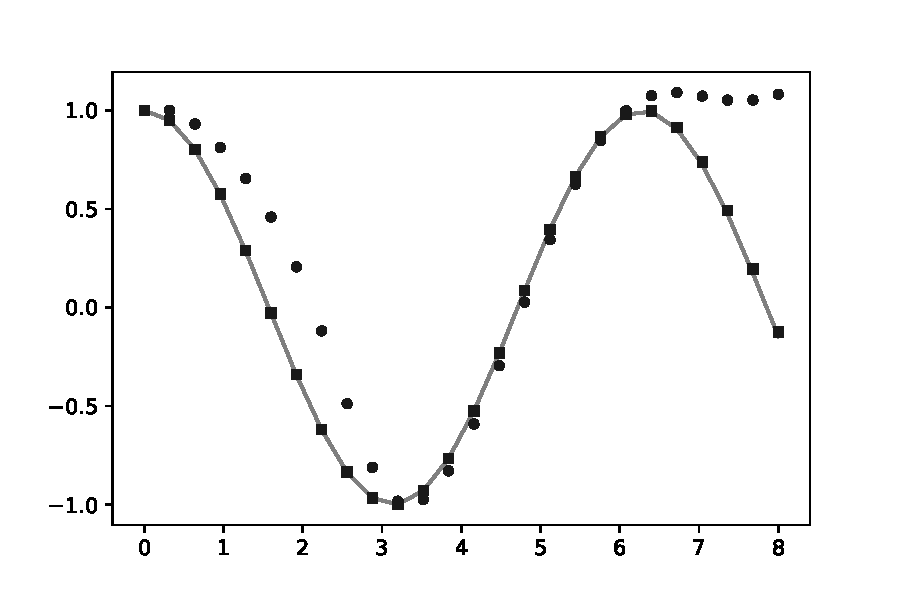
\includegraphics[width=\textwidth]{img/5/N25.pdf}
    \caption{computed solutions with \( N = 25 \) mesh points}
\end{subfigure}
\begin{subfigure}{.48\textwidth}
    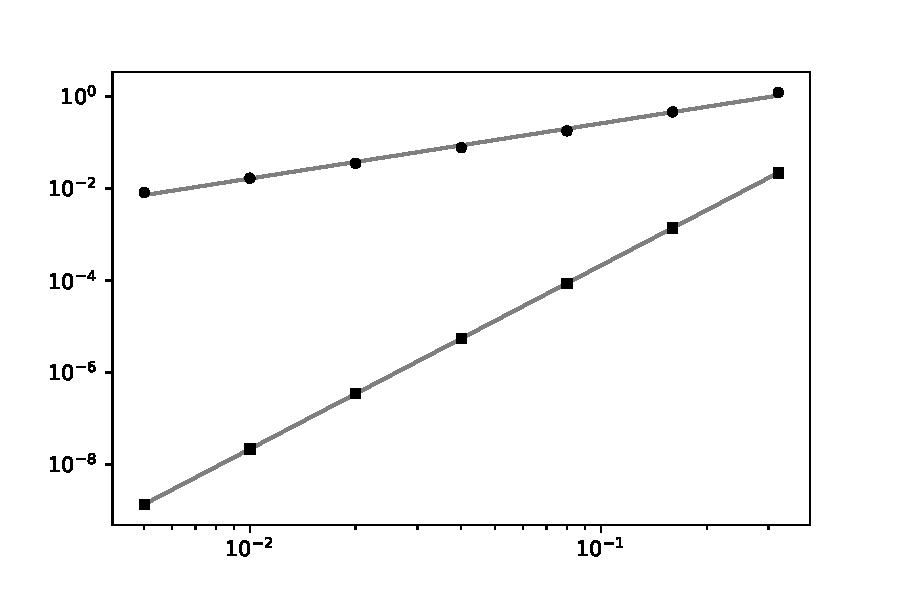
\includegraphics[width=\textwidth]{img/5/error.pdf}
    \caption{infinity norm of error vs mesh spacing}
\end{subfigure}
\caption{circle: Forward Euler, square: Runge-Kutta}
\label{p5}
\end{figure}


\end{solution}

\begin{problem}[Problem 6]
Use a method of your choice or try \verb+ode45+ in Matlab to solve the Lotka-Volterra predator-prey
equations:
\begin{eqnarray*}
R' & = & (1 - .02F) R , \\
F' & = & (-1 + .03R) F ,
\end{eqnarray*}
starting with \( R_0 = F_0 = 20 \).  Plot \( R(t) \) and \( F(t) \) vs. t on the same plot, labeling each curve.
Present the solution in another way with a plot of \( F \) vs. \( R \).
\end{problem}

\begin{solution}[Solution]

We implement this using Scipy's IVP solver, requring it to use the eplicit Runge-Kutta method of order 5(4). According to the documentation, ``The error is controlled assuming 4th order accuracy, but steps are taken using a 5th oder accurate formula (local extrapolation is done).'' The right hand side function is define inline as a lambda function.
\lstinputlisting[linerange=\#<startTeX>-\#<endTeX>]{hw1_6.py}

The outputs \( R \) and \( F \) are plotted against time in Figure~\ref{vs} and against eachother in Figure~\ref{phase}. The solution is periodic which is seen in the closed contour of the phase portrait. We run the solver from time 0 to 20 which covers about three cycles.
\begin{figure}[H]\centering
    \begin{subfigure}{.48\textwidth}
        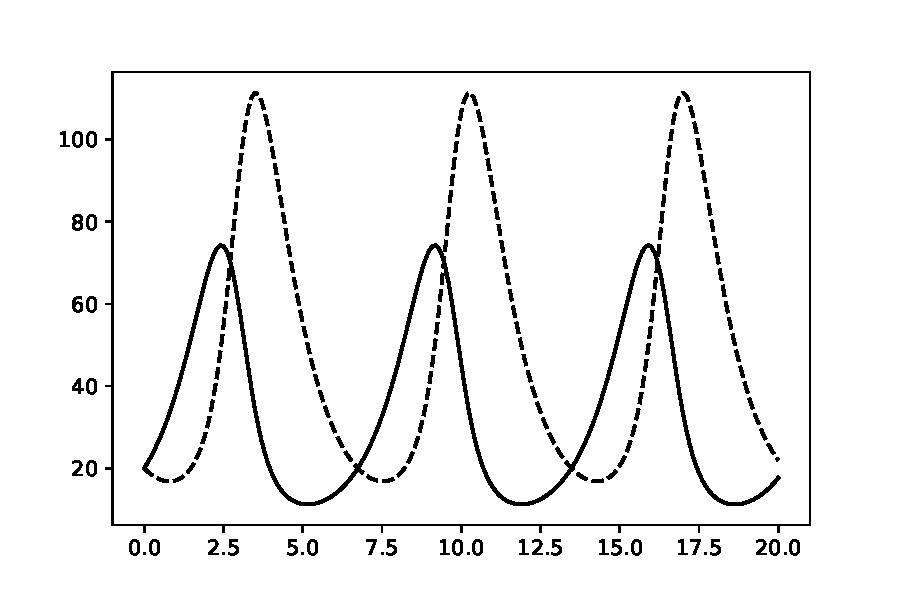
\includegraphics[width=\textwidth]{img/6/solution.pdf}
        \caption{solid: \( R \), dashed: \( F \)}
        \label{vs}
    \end{subfigure}
    \begin{subfigure}{.48\textwidth}
        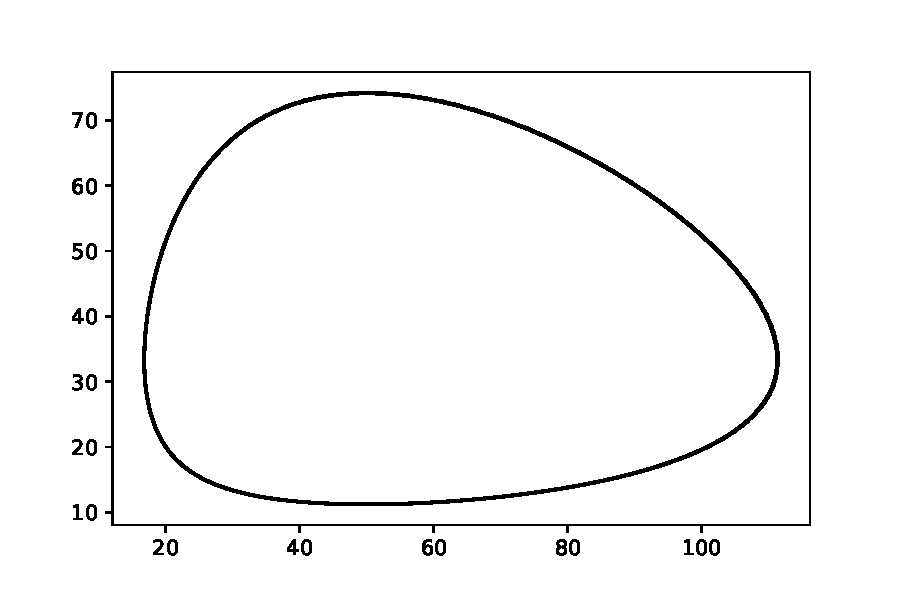
\includegraphics[width=\textwidth]{img/6/phase.pdf}
        \caption{\( F \) vs. \( R \)}
        \label{phase}
    \end{subfigure}
    \caption{output of RK45 solver on give IVP}
    \label{p6}
\end{figure}

\end{solution}

\end{document}
